%% LyX 2.1.2 created this file.  For more info, see http://www.lyx.org/.
%% Do not edit unless you really know what you are doing.
\documentclass[american,fontsize=11pt,paper=a4,twoside,openright,titlepage,numbers=noenddot,headinclude,BCOR=5mm,footinclude=true,cleardoublepage=empty]{scrreprt}
\usepackage[T1]{fontenc}
\setcounter{secnumdepth}{2}
\usepackage{graphicx}
\usepackage[numbers]{natbib}

\makeatletter

%%%%%%%%%%%%%%%%%%%%%%%%%%%%%% LyX specific LaTeX commands.
%% A simple dot to overcome graphicx limitations
\newcommand{\lyxdot}{.}


%%%%%%%%%%%%%%%%%%%%%%%%%%%%%% Textclass specific LaTeX commands.
% Classic Thesis Style loader
\makeatother
\input{classicthesis-config.tex}
\makeatletter
% use Latin Modern instead of Computer Modern sans serif
\renewcommand{\sfdefault}{lmss}

\makeatother

\usepackage{babel}
\begin{document}

\section{Introduction to Hydrofracturing \label{sec:Literature-overview}}

To begin, lets start with a brief explanation of what hydrofracturing
is, and why it was created. Natural gas and oil are the main fossil
fuels in use for over a century. These were initially extracted from
conventional deposits, underground pockets of trapped hydrocarbons.
Figure \ref{gas_picture} shows various types of oil and gas reservoirs,
where an example of conventional gas deposit is shown. These deposits
were relatively easy to access, when a rig was drilled the pressure
would often force a violate burst of stored fissile fuel. A very accurate
(and somehow over dramatic) cinematization of these early days oil
industry could even be seen in a number of Hollywood productions \citep{there_will_be_blood}.
Even in recent history there are examples of oil and gas uncontrollably
forcing its way to the surface: 1991 Kuwait and 2010 Gulf of Mexico,
to name just a few major ones. It could be mistaken that extraction
of liquid fossil fuels is just about capturing this uncontrollable
flow of free natural resource. 

Unfortunately, is reality oil and gas acquisition a complex multiphysics
problem. In an attempt to introduce the overall complexity, lets begin
with pressure, porosity and permeability . As anyone should recall,
the deeper underground we go the higher the pressure, at depths of
a few kilometers this will be a multitude of the atmospheric pressure.
Porosity is a measure of how much of a rock is open space, a proportion
of pores to solid matter {[}ref to google ?{]}, and even at these
great depths, there pores might be filled with some hydrocarbonate
fluid. Finally Permeability is a measure of the ease with which a
fluid (oil or gas) can move through a porous rock. A conventional
reservoir would therefore be made of a filled porous rock, such as
sandstone, covered by some other impermeable rock layer. The drilled
well would create a path that would allow a pressure driven viscous
flow of oil or gas to the surface, which could be modeled by modeled
by Darcy's Law \citep{darcy_law}. These type of reservoirs are still
operational, and contribute to a major part of the worlds oil and
gas production, however many are depleted or running dry.

\begin{figure}
\label{gas_picture}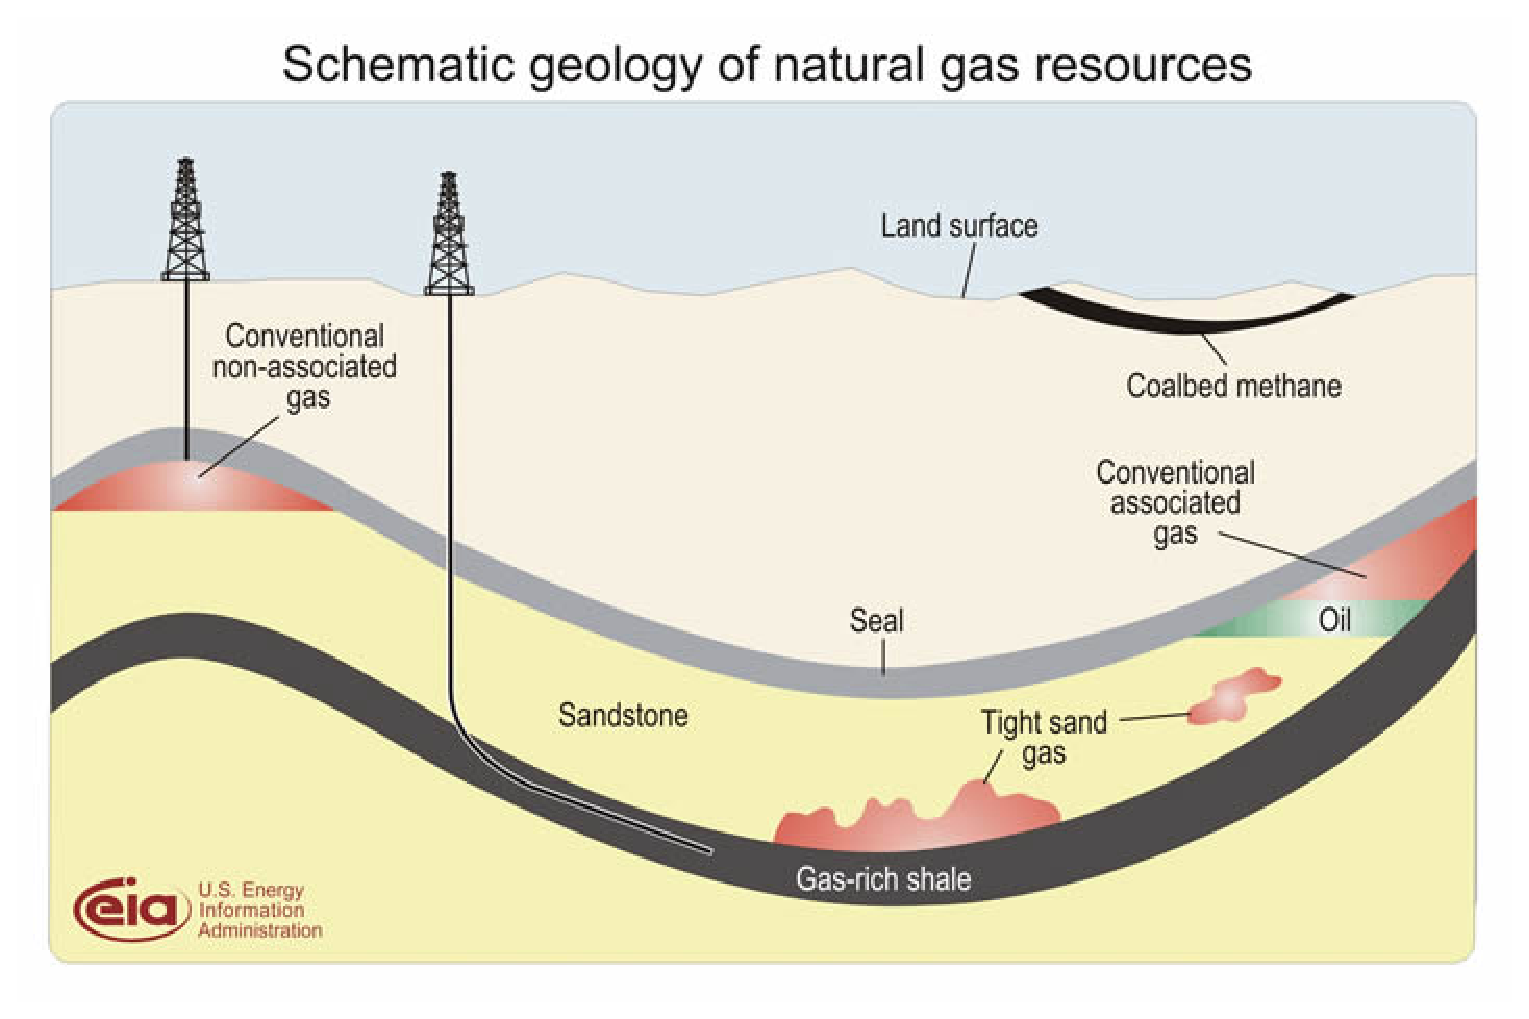
\includegraphics[scale=0.5]{GasDepositDiagram}\protect\caption{Schematic geology of natural gas resources (source \citep{wiki_natural_gass})}
\end{figure}


\clearpage

The output of conventional oil and gas fields could be described by
Hubbert Curve \citep{Hubbert1}, a model that assumes some peek in
production followed by a steady decline. In the US (see Figure \ref{oil_peak_fig})
these maximum production output would occur in 1970s. Thou as known
techniques of hydrocarbons extraction were proving to be insufficient,
efforts to find new way of obtaining oil were made. The first pioneering
papers on the topic of hydrofracturing \citep{Crittendon,Geertsma,Harrison,Hubbert,Khristianovic,Nordgren,Perkins,SS}
were published during that time period, as the industry realized the
need to use new, unconventional methods of hydrocarbon recovery to
meet the growing supply.

\begin{figure}
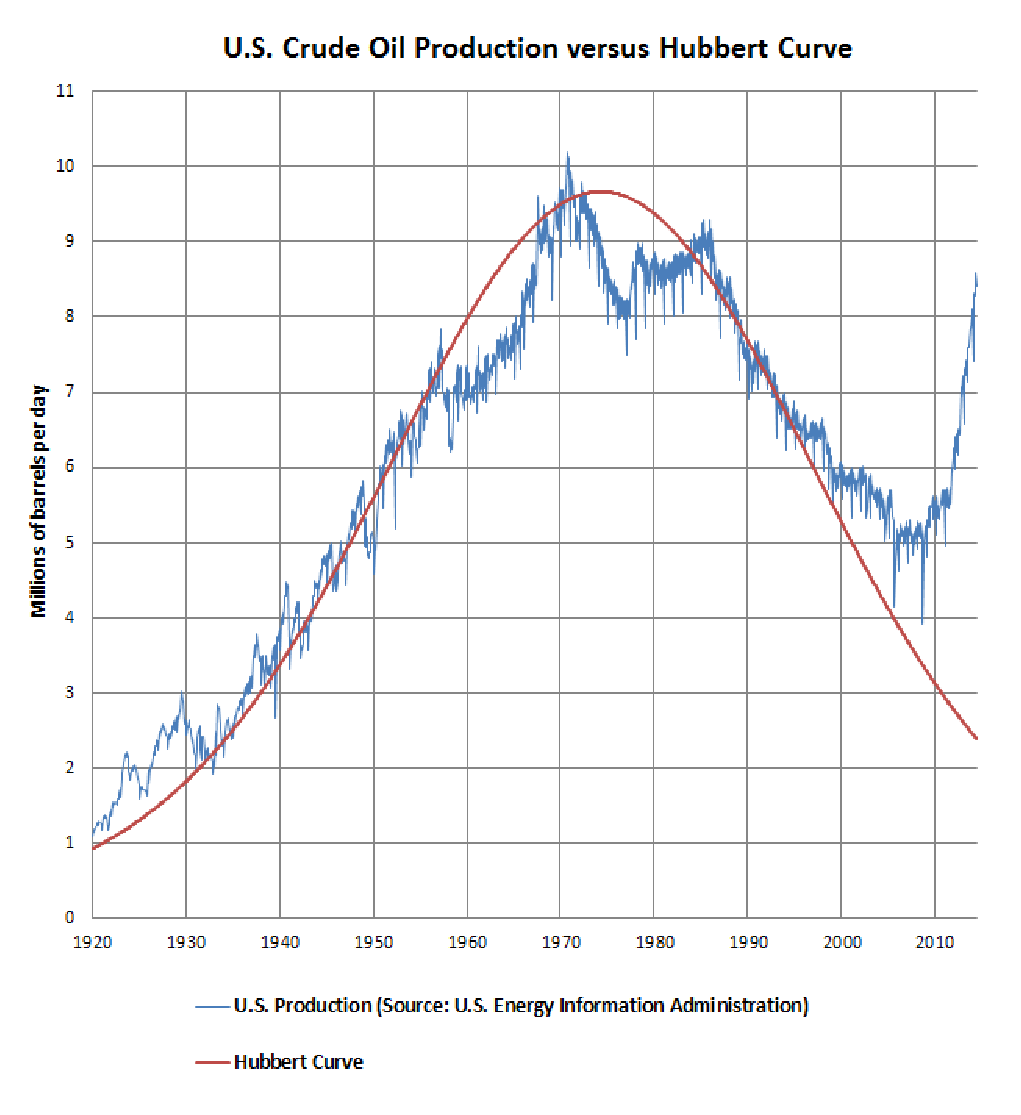
\includegraphics[scale=0.6]{US_Crude_Oil_Production_versus_Hubbert_Curve}\label{oil_peak_fig}\protect\caption{Oil production in USA throughout past century (source \citep{wiki_peak_oil})}
\end{figure}


\clearpage

In its broadest definition, \emph{hydraulic fracturing refers to a
problem of a fluid driven fracture propagating in a brittle medium}.
It is a naturally occurring process observable in formation of magma
dykes \citep{Rubin,Lister,Lister_Kerr} or subglacial drainage of
water \citep{Rice}. The possible applications also go beyond petroleum
industry: disposal of waste drill cuttings underground \citep{Moschovidis},
geothermal reservoirs exploitation \citep{Pine} or coalbeded methane
extraction. It is not the only reservoir stimulation method available,
some other techniques involve washing away renaming fossil fuels with
specially prepared foam \citep{simon}. A typical fracturing job,
as shown on Figure \ref{fracking_scheme}, could be done in the following
stages:
\begin{itemize}
\item Drilling of a vertical well, or preparation of existing one if stimulating
depleted reservoir. The wells walls must be prepared to withstand
massive pressures without unanticipated leak go the ground waters. 
\item Drilling of a long horizontal section that spams through target resource
rich rock formation, which could be gas rich shale as shown on Figure
\ref{gas_picture}. It is a fairly recent technique that requires
proper drilling heads. 
\item Preparation of initial fractures with directed explosive charges.
\item Pumping of fracturing fluid. This could go on for days, and requires
substantial reserves of water, chemical additives, and powerful pumps.
\item Mixing in proppant, to support created fractures from closing. Sand,
or other granulate such as ceramic grains.
\item And finally moving on to production phase.
\end{itemize}
The process is indeed very sophisticated and expensive, but pays off.
Due to its application, the Hubbert Curve has been beaten \citep{Cavallo}
and the popularized in mass media forecast of fossil fuel depletion
appears to be postponed at least to the next century. Indeed over
the past decade natural gas production in the US alone increased by
over 50\% \citep{usa_gas_production} due to recent shale gas boom.
This was achieved thanks to hydrofracturing. Shale gas deposits, as
opposed to conventional sandstones, have natural gas trapped in pores
off non permeable shale formations (see Figure \ref{gas_picture}
again). Hydrofracturing, pumping fluid under extremely high pressures
opens new fractures, and creates pathways for the natural gas to escape
pores in shale and flow to the surface.

This work should cover only a single stage of the hydrofracturing
process, the numerical modeling of fracture propagation due to fluid
pumping. Although it is only one stage of the whole multiphysics problem,
it is already a sufficient challenge on its own. The previous physical
concepts: pressure, porosity and permeability of the reservoir now
will coupled with incompressible viscous fluid dynamics, fracture
mechanic and complex non static geometries into a dynamic mathematical
model. This will cover the evolution of short initial fractures located
right at the drilled wellbore, to an underground system of multiple
fractures, that could spam over several kilometers. The engineering
and geological challenges of choosing right drilling place, preparing
a sufficient horizontal well at depths of up to a few kilometers,
and maintaining later production will not be covered here. Similarity
the problem of proppant mixing, that follows immediately after the
stage of fracture propagation will not be mentioned here, as it would
introduce even more physical properties, and extend the overall complexity
beyond manageable level. Even the oldest and relatively simple proppant
model by Einstein \citep{Einstein}, could not describe the actual
physical process correctly \citep{Kuzkin}, but would introduce another
problem of changing fluid viscosity, not to mention other thermal
and chemical processes, that could affect fracture propagation. 

\begin{figure}
\includegraphics[scale=0.5]{737px-HydroFrac2\lyxdot svg}\label{fracking_scheme}\protect\caption{A schematics of hydrofracturing job (source \citep{wiki_fracturing})}
\end{figure}

\end{document}
